%% uncomment to list all files in log
%\listfiles

\documentclass[12pt]{report}


\usepackage{fontspec}

%\setmainfont[Scale=MatchLowercase]{Lucida Bright}
%\setmonofont{FreeMono}
%\setmonofont{Source Code Pro}
\setmonofont[Scale=MatchLowercase]{Ubuntu Mono}

\usepackage[headings]{fullpage}

% national use characters 
%\usepackage{inputenc}

% ams mathematical symbols
\usepackage{amsmath,amssymb}

% added to support pandoc highlighting
\usepackage{microtype}

\usepackage{makeidx}

% add index and bibliographies to table of contents
\usepackage[nottoc]{tocbibind}

% postscript courier and times in place of cm fonts
%\usepackage{courier}
%\usepackage{times}

% extended coloring
\usepackage{color}
\usepackage[table,dvipsnames]{xcolor}
\usepackage{colortbl}

% advanced date formating
\usepackage{datetime}

%support pandoc code highlighting
\usepackage{fancyvrb}
\DefineShortVerb[commandchars=\\\{\}]{\|}
\DefineVerbatimEnvironment{Highlighting}{Verbatim}{commandchars=\\\{\}}
% Add ',fontsize=\small' for more characters per line

%tango style colors
% \usepackage{framed}
% \definecolor{shadecolor}{RGB}{255,255,255}
% \newenvironment{Shaded}{\begin{snugshade}}{\end{snugshade}}
% \newcommand{\KeywordTok}[1]{\textcolor[rgb]{0.13,0.29,0.53}{\textbf{{#1}}}}
% \newcommand{\DataTypeTok}[1]{\textcolor[rgb]{0.13,0.29,0.53}{{#1}}}
% \newcommand{\DecValTok}[1]{\textcolor[rgb]{0.00,0.00,0.81}{{#1}}}
% \newcommand{\BaseNTok}[1]{\textcolor[rgb]{0.00,0.00,0.81}{{#1}}}
% \newcommand{\FloatTok}[1]{\textcolor[rgb]{0.00,0.00,0.81}{{#1}}}
% \newcommand{\CharTok}[1]{\textcolor[rgb]{0.31,0.60,0.02}{{#1}}}
% \newcommand{\StringTok}[1]{\textcolor[rgb]{0.31,0.60,0.02}{{#1}}}
% \newcommand{\CommentTok}[1]{\textcolor[rgb]{0.56,0.35,0.01}{\textit{{#1}}}}
% \newcommand{\OtherTok}[1]{\textcolor[rgb]{0.56,0.35,0.01}{{#1}}}
% \newcommand{\AlertTok}[1]{\textcolor[rgb]{0.94,0.16,0.16}{{#1}}}
% \newcommand{\FunctionTok}[1]{\textcolor[rgb]{0.00,0.00,0.00}{{#1}}}
% \newcommand{\RegionMarkerTok}[1]{{#1}}
% \newcommand{\ErrorTok}[1]{\textbf{{#1}}}
% \newcommand{\NormalTok}[1]{{#1}}

%espresso style colors
% \usepackage{framed}
% \definecolor{shadecolor}{RGB}{42,33,28}
% \newenvironment{Shaded}{\begin{snugshade}}{\end{snugshade}}
% \newcommand{\KeywordTok}[1]{\textcolor[rgb]{0.26,0.66,0.93}{\textbf{{#1}}}}
% \newcommand{\DataTypeTok}[1]{\textcolor[rgb]{0.74,0.68,0.62}{\underline{{#1}}}}
% \newcommand{\DecValTok}[1]{\textcolor[rgb]{0.27,0.67,0.26}{{#1}}}
% \newcommand{\BaseNTok}[1]{\textcolor[rgb]{0.27,0.67,0.26}{{#1}}}
% \newcommand{\FloatTok}[1]{\textcolor[rgb]{0.27,0.67,0.26}{{#1}}}
% \newcommand{\CharTok}[1]{\textcolor[rgb]{0.02,0.61,0.04}{{#1}}}
% \newcommand{\StringTok}[1]{\textcolor[rgb]{0.02,0.61,0.04}{{#1}}}
% \newcommand{\CommentTok}[1]{\textcolor[rgb]{0.00,0.40,1.00}{\textit{{#1}}}}
% \newcommand{\OtherTok}[1]{\textcolor[rgb]{0.74,0.68,0.62}{{#1}}}
% \newcommand{\AlertTok}[1]{\textcolor[rgb]{1.00,1.00,0.00}{{#1}}}
% \newcommand{\FunctionTok}[1]{\textcolor[rgb]{1.00,0.58,0.35}{\textbf{{#1}}}}
% \newcommand{\RegionMarkerTok}[1]{\textcolor[rgb]{0.74,0.68,0.62}{{#1}}}
% \newcommand{\ErrorTok}[1]{\textcolor[rgb]{0.74,0.68,0.62}{\textbf{{#1}}}}
% \newcommand{\NormalTok}[1]{\textcolor[rgb]{0.74,0.68,0.62}{{#1}}}

%kete style colors
% \newenvironment{Shaded}{}{}
% \newcommand{\KeywordTok}[1]{\textbf{{#1}}}
% \newcommand{\DataTypeTok}[1]{\textcolor[rgb]{0.50,0.00,0.00}{{#1}}}
% \newcommand{\DecValTok}[1]{\textcolor[rgb]{0.00,0.00,1.00}{{#1}}}
% \newcommand{\BaseNTok}[1]{\textcolor[rgb]{0.00,0.00,1.00}{{#1}}}
% \newcommand{\FloatTok}[1]{\textcolor[rgb]{0.50,0.00,0.50}{{#1}}}
% \newcommand{\CharTok}[1]{\textcolor[rgb]{1.00,0.00,1.00}{{#1}}}
% \newcommand{\StringTok}[1]{\textcolor[rgb]{0.87,0.00,0.00}{{#1}}}
% \newcommand{\CommentTok}[1]{\textcolor[rgb]{0.50,0.50,0.50}{\textit{{#1}}}}
% \newcommand{\OtherTok}[1]{{#1}}
% \newcommand{\AlertTok}[1]{\textcolor[rgb]{0.00,1.00,0.00}{\textbf{{#1}}}}
% \newcommand{\FunctionTok}[1]{\textcolor[rgb]{0.00,0.00,0.50}{{#1}}}
% \newcommand{\RegionMarkerTok}[1]{{#1}}
% \newcommand{\ErrorTok}[1]{\textcolor[rgb]{1.00,0.00,0.00}{\textbf{{#1}}}}
% \newcommand{\NormalTok}[1]{{#1}}
%end pandoc code hacks

% jodliterate colors
\usepackage{color}
\definecolor{shadecolor}{RGB}{248,248,248}
% j control structures 
\definecolor{keywcolor}{rgb}{0.13,0.29,0.53}
% j explicit arguments x y m n u v
\definecolor{datacolor}{rgb}{0.13,0.29,0.53}
% j numbers - all types see j.xml
\definecolor{decvcolor}{rgb}{0.00,0.00,0.81}
\definecolor{basencolor}{rgb}{0.00,0.00,0.81}
\definecolor{floatcolor}{rgb}{0.00,0.00,0.81}
% j local assignments
\definecolor{charcolor}{rgb}{0.31,0.60,0.02}
\definecolor{stringcolor}{rgb}{0.31,0.60,0.02}
\definecolor{commentcolor}{rgb}{0.56,0.35,0.01}
% primitive adverbs and conjunctions
%\definecolor{othercolor}{rgb}{0.56,0.35,0.01}   
\definecolor{othercolor}{RGB}{0,0,255}
% global assignments
\definecolor{alertcolor}{rgb}{0.94,0.16,0.16}
% primitive J verbs and noun names
\definecolor{funccolor}{rgb}{0.00,0.00,0.00}    

\usepackage{framed}
\newenvironment{Shaded}{}{}
\newcommand{\KeywordTok}[1]{\textcolor{keywcolor}{\textbf{{#1}}}}
\newcommand{\DataTypeTok}[1]{\textcolor{datacolor}{{#1}}}
%\newcommand{\DecValTok}[1]{\textcolor{decvcolor}{{#1}}}
\newcommand{\DecValTok}[1]{{#1}} 
\newcommand{\BaseNTok}[1]{\textcolor{basencolor}{{#1}}}
\newcommand{\FloatTok}[1]{\textcolor{floatcolor}{{#1}}}
\newcommand{\CharTok}[1]{\textcolor{charcolor}{\textbf{{#1}}}}
\newcommand{\StringTok}[1]{\textcolor{stringcolor}{{#1}}}
\newcommand{\CommentTok}[1]{\textcolor{commentcolor}{\textit{{#1}}}}
\newcommand{\OtherTok}[1]{\textcolor{othercolor}{{#1}}} 
\newcommand{\AlertTok}[1]{\textcolor{alertcolor}{\textbf{{#1}}}}
%\newcommand{\FunctionTok}[1]{\textcolor{funccolor}{{#1}}}
\newcommand{\FunctionTok}[1]{{#1}}
\newcommand{\RegionMarkerTok}[1]{{#1}}
\newcommand{\ErrorTok}[1]{\textbf{{#1}}}
\newcommand{\NormalTok}[1]{{#1}}

% headers and footers
\usepackage{fancyhdr}
\pagestyle{fancy}

\fancyhead{}
\fancyfoot{}

%\fancyhead[LE,RO]{\slshape \rightmark}
%\fancyhead[LO,RE]{\slshape \leftmark}
\fancyfoot[C]{\thepage}
%\headrulewidth 0.4pt
%\footrulewidth 0 pt

%\addtolength{\headheight}{\baselineskip}

%\lfoot{\emph{Analyze the Data not the Drivel}}
%\rfoot{\emph{\today}}

% subfigure handles figures that contain subfigures
%\usepackage{color,graphicx,subfigure,sidecap}
\usepackage{graphicx,sidecap}
\usepackage{subfigure}
\graphicspath{{./inclusions/}}

% floatflt provides for text wrapping around small figures and tables
\usepackage{floatflt}

% tweak caption formats 
\usepackage{caption} 
\usepackage{sidecap}
%\usepackage{subcaption} % not compatible with subfigure

\usepackage{rotating} % flip tables sideways

% complex footnotes
%\usepackage{bigfoot}

% weird logos \XeLaTeX
\usepackage{metalogo}

% source code listings
\usepackage{listings}

% long tables
% \usepackage{longtable}

\newcommand{\HRule}{\rule{\linewidth}{0.5mm}}

% map LaTeX cross references into PDF cross references
\usepackage[
            %dvips,
            colorlinks,
            linkcolor=blue,
            citecolor=blue,
            urlcolor=blue,   % magenta, cyan default        
            pdfauthor={John D. Baker},
            pdftitle={Analyze the Data not the Drivel},
            pdfsubject={Blog},
            pdfcreator={MikTeX+LaTeXe with hyperref package},
            pdfkeywords={blog,wordpress},
            ]{hyperref}
           
% custom colors
\definecolor{CodeBackGround}{cmyk}{0.0,0.0,0,0.05}    % light gray
\definecolor{CodeComment}{rgb}{0,0.50,0.00}           % dark green {0,0.45,0.08}
\definecolor{TableStripes}{gray}{0.9}                 % odd/even background in tables

\lstdefinelanguage{bat}
{morekeywords={echo,title,pushd,popd,setlocal,endlocal,off,if,not,exist,set,goto,pause},
sensitive=True,
morecomment=[l]{rem}
}

\lstdefinelanguage{jdoc}
{
morekeywords={},
otherkeywords={assert.,break.,continue.,for.,do.,if.,else.,elseif.,return.,select.,end.
,while.,whilst.,throw.,catch.,catchd.,catcht.,try.,case.,fcase.},
sensitive=True,
morecomment=[l]{NB.},
morestring=[b]',
morestring=[d]',
}

% latex size ordering - can never remember it
% \tiny
% \scriptsize
% \footnotesize
% \small
% \normalsize
% \large
% \Large
% \LARGE
% \huge
% \Huge
 
% listings package settings  
\lstset{%
  language=jdoc,                                % j document settings
  basicstyle=\ttfamily\footnotesize,            
  keywordstyle=\bfseries\color{keywcolor}\footnotesize,
  identifierstyle=\color{black},
  commentstyle=\slshape\color{CodeComment},     % colored slanted comments
  stringstyle=\color{red}\ttfamily,
  showstringspaces=false,                       
  %backgroundcolor=\color{CodeBackGround},       
  frame=single,                                
  framesep=1pt,                                 
  framerule=0.8pt,                             
  rulecolor=\color{CodeBackGround},   
  showspaces=false,
  %columns=fullflexible,
  %numbers=left,
  %numberstyle=\footnotesize,
  %numbersep=9pt,
  tabsize=2,
  showtabs=false,
  captionpos=b
  breaklines=true,                              
  breakindent=5pt                              
}

\lstdefinelanguage{JavaScript}{
  keywords={typeof, new, true, false, catch, function, return, null, catch, switch, var, if, in, while, do, else, case, break},
  ndkeywords={class, export, boolean, throw, implements, import, this},
  ndkeywordstyle=\color{darkgray}\bfseries,
  sensitive=false,
  comment=[l]{//},
  morecomment=[s]{/*}{*/},
  morestring=[b]',
  morestring=[b]"
}

% C# settings
\lstdefinestyle{sharpc}{
language=[Sharp]C,
basicstyle=\ttfamily\scriptsize, 
keywordstyle=\bfseries\color{keywcolor}\scriptsize,
framerule=0pt
}

% for source code listing longer than two use smaller font
\lstdefinestyle{smallersource}{
basicstyle=\ttfamily\scriptsize, 
keywordstyle=\bfseries\color{keywcolor}\scriptsize,
framerule=0pt
}

\lstdefinestyle{resetdefaults}{
language=jdoc,
basicstyle=\ttfamily\footnotesize,  
keywordstyle=\bfseries\color{keywcolor}\footnotesize,                                                               
framerule=0.8pt 
}

% APL UTF8 code points listed for lstlisting processing
\makeatletter
\lst@InputCatcodes
\def\lst@DefEC{%
 \lst@CCECUse \lst@ProcessLetter
  ^^80^^81^^82^^83^^84^^85^^86^^87^^88^^89^^8a^^8b^^8c^^8d^^8e^^8f%
  ^^90^^91^^92^^93^^94^^95^^96^^97^^98^^99^^9a^^9b^^9c^^9d^^9e^^9f%
  ^^a0^^a1^^a2^^a3^^a4^^a5^^a6^^a7^^a8^^a9^^aa^^ab^^ac^^ad^^ae^^af%
  ^^b0^^b1^^b2^^b3^^b4^^b5^^b6^^b7^^b8^^b9^^ba^^bb^^bc^^bd^^be^^bf%
  ^^c0^^c1^^c2^^c3^^c4^^c5^^c6^^c7^^c8^^c9^^ca^^cb^^cc^^cd^^ce^^cf%
  ^^d0^^d1^^d2^^d3^^d4^^d5^^d6^^d7^^d8^^d9^^da^^db^^dc^^dd^^de^^df%
  ^^e0^^e1^^e2^^e3^^e4^^e5^^e6^^e7^^e8^^e9^^ea^^eb^^ec^^ed^^ee^^ef%
  ^^f0^^f1^^f2^^f3^^f4^^f5^^f6^^f7^^f8^^f9^^fa^^fb^^fc^^fd^^fe^^ff%
  ^^^^20ac^^^^0153^^^^0152%
  ^^^^20a7^^^^2190^^^^2191^^^^2192^^^^2193^^^^2206^^^^2207^^^^220a%
  ^^^^2218^^^^2228^^^^2229^^^^222a^^^^2235^^^^223c^^^^2260^^^^2261%
  ^^^^2262^^^^2264^^^^2265^^^^2282^^^^2283^^^^2296^^^^22a2^^^^22a3%
  ^^^^22a4^^^^22a5^^^^22c4^^^^2308^^^^230a^^^^2336^^^^2337^^^^2339%
  ^^^^233b^^^^233d^^^^233f^^^^2340^^^^2342^^^^2347^^^^2348^^^^2349%
  ^^^^234b^^^^234e^^^^2350^^^^2352^^^^2355^^^^2357^^^^2359^^^^235d%
  ^^^^235e^^^^235f^^^^2361^^^^2362^^^^2363^^^^2364^^^^2365^^^^2368%
  ^^^^236a^^^^236b^^^^236c^^^^2371^^^^2372^^^^2373^^^^2374^^^^2375%
  ^^^^2377^^^^2378^^^^237a^^^^2395^^^^25af^^^^25ca^^^^25cb%  
  ^^00}
\lst@RestoreCatcodes
\makeatother

% custom lengths used within minipages
\newcommand{\minindent}{17pt}


\makeindex

\begin{document}

\subsection*{\href{https://bakerjd99.wordpress.com/2013/08/05/the-new-smugmug/}{The New SmugMug}}
\addcontentsline{toc}{subsection}{The New SmugMug}


\noindent\emph{Posted: 06 Aug 2013 04:55:48}
\vspace{6pt}

Websites compete in a brutal Darwinian struggle for eyeballs and clicks:
adapt or die is an understatement. Every few years users get
``upgraded'' whether they want it or not. Generally things move in a
better direction. Even twenty-something web programmers aren't
completely stupid but setbacks and complete disasters are not uncommon.


%{[}caption id=``attachment\_4141'' align=``aligncenter''  width=``350''{]}
%\href{http://conceptcontrol.smugmug.com/}{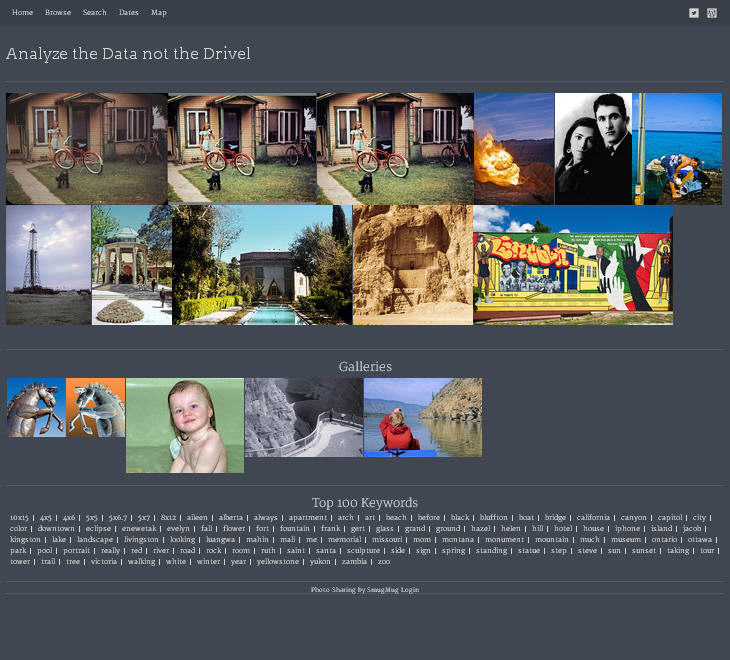
\includegraphics{newsmugss.jpg}}
%My new SmugMug layout - click to view.
%{[}/caption{]}

\captionsetup[figure]{labelformat=empty}
\captionsetup[floatingfigure]{labelformat=empty}

\begin{floatingfigure}[r]{0.37\textwidth}
%\begin{figure}[htbp]
\centering
\href{http://conceptcontrol.smugmug.com/}{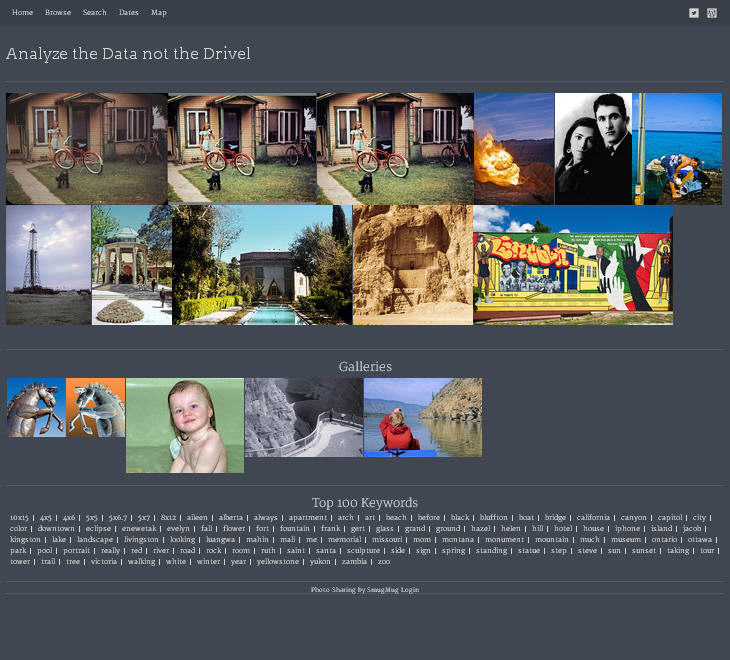
\includegraphics[width=0.32\textwidth]{newsmugss.jpg}}
\caption{My new SmugMug layout.}
\label{fig:4126X0}
%\end{figure}
\end{floatingfigure}


My relationship with \href{http://www.smugmug.com/}{SmugMug} started
about five years ago when my \href{http://www.flickr.com/}{Flickr}
account was suddenly declared ``mature'' by some faceless administrative
ape that couldn't tell the difference between innocent nudes and
pornography. I was so incensed I sent Flickr administrators a message
they couldn't ignore. I painstakingly deleted all my images, mass
deletion was oddly not supported by the
\href{http://www.yahoo.com/}{Yahoo's} that ran the joint, and dropped my
account. How's that for maturity? I consider it my sacred duty to punish
companies that screw customers. After dumping Flickr I searched around
and found SmugMug.

There were things I liked and didn't like about SmugMug. SmugMug did a
better job of displaying images than Flickr and you could select your
\emph{own} damn background color. On the downside, SmugMug has more of
an empty art museum vibe than Flickr's busy social whorehouse milieu.
For a few days I missed complete morons dropping snide asides on my
pictures. The only comments I get on SmugMug come from family members
and energetic strangers that find something they like enough to breach
SmugMug's spam fortifications. The silence is welcome. This is an art
museum after all.

SmugMug offers a number of account types. I am a ``power'' user. A power
account falls between basic and pro accounts. This account
differentiation makes sense. SmugMug users fall into three classes.

\begin{enumerate}
\item
  \textbf{Basic:} plain folks that want a no fuss picture website.
\item
  \textbf{Power:} nondelusional keen photographers.
\item
  \textbf{Pro:} delusional ``serious'' photographers.
\end{enumerate}

Only paparazzi, porn, wedding, fashion, sports and National Geographic
photographers are making any money taking pictures these days. If you
don't fall into any of these classes my guess is that you are spending
more on photography than you are making. SmugMug harbors
many photographers attempting to sell their pictures. I would never buy
a picture nor would I expect to sell one. I see many shots on sale that
aren't as good as many I've made for free. There are billions of cameras
in the wild these days. Photography is not exempt from the law of supply
and demand. When the supply is nearly infinite what do you expect the
price to be? This is why newspapers are laying off staff photographers
and small photography studios have mostly gone out of business. As a
keen amateur photographer this saddens me but as a right-wing
libertarian death beast it warms my dark evil heart that most of the
``photographers'' being discarded are rent seeking nitwits playing
\href{http://www.magnumphotos.com/C.aspx?VP3=CMS3\&VF=MAGO31\_10\_VForm\&ERID=24KL53ZMYN}{Henri
Cartier-Bresson.} Still photography is no longer a viable personal
business! We're deep into another age people. Now that you see where I'm
coming from let's get on with what's good and bad about the new SmugMug.

\medskip

Let's start with the good stuff:

\begin{enumerate}
\item
  \textbf{Stretchy layouts:} The new website does a better job of
  automatically adapting to a variety of display devices. I've browsed
  \href{http://conceptcontrol.smugmug.com/}{my own site} on phones,
  tablets, laptops and giant desktop displays. It looks OK on all of
  them and great on tablets and laptops.
\item
  \textbf{Easy customization and layout tweaking:} It took me all of ten
  minutes to figure out the new layout controls. Programming \emph{easy
  nontrivial} customization is hard. Here the SmugMug programmers have
  brilliantly succeeded. I know enough about JavaScript, CSS and HTML to
  roll my own designs but photography is a hobby; I'd rather spend my
  time taking and refining pictures that writing JavaScript to display
  them.
\item
  \textbf{Better overall site organization:} The new site organizer is a
  significant improvement on older methods and allowing deeper directory
  paths will be appreciated by many.
\item
  \textbf{An improved and better integrated mapping facility:}
  Displaying geotagged images on old SmugMug was somewhat jarring. The
  control was clunky and it didn't match your site design. The new
  control adapts to your layout and ``circle'' area browsing is slick
  and intuitive.
\end{enumerate}

Now for the dark side:

\begin{enumerate}
\item
  \textbf{Website migration has hiccups:} My site has over two thousands
  images. I didn't expect the migration to the new layout to be without
  problems and it wasn't. For me the biggest problem was the handling of
  keywords. The new site does not properly display keyword strings if
  the ``;'' delimiter is used. I have thousands of pictures with
  ``keywords'' like:

\begin{verbatim}
    5x5;capillary;glass;microscope;polywater;ultra;
\end{verbatim}

  The ``;'' character delimits separate words. It should be displayed
  like:

\begin{verbatim}
    5x5 | capillary | glass | microscope | polywater | ultra
\end{verbatim}

  When you click on the ``;'' string it is interpreted as a ``find all
  images with all these keywords'' request which is usually the very
  image you are browsing. This is mostly a display problem. The
  individual keywords were properly parsed and loaded.
\item
  \textbf{Custom API applications break:} I use a custom application I
  wrote to synchronize my SmugMug online galleries with my offline
  \href{http://www.cerious.com/}{ThumbsPlus} databases. This application
  issues SmugMug REST API calls to collect and update image metadata.
  When I migrated I expected this application to stop working and it
  did. It looks like I need to authenticate my application with the new
  SmugMug site. There are no \emph{easily found instructions} on how to
  do this. I hope this is just an oversight and that power users can
  still run custom API applications.
\item
  \textbf{The new map control is limited to one hundred images:} The
  slick circle browser map control will only display one hundred images
  and there is no easy way to set it to map pictures in a particular
  gallery. The old clunky control allowed two hundred pictures and it
  could display arbitrary galleries.
\end{enumerate}

I could go on but I program for a living. I know users always whine
about change and seldom express gratitude for all the hard work the code
monkeys of the world do to keep the lights on. Overall the new SmugMug
is better than the old. There are problems but for a first production
cut this is fine work. It certainly merits one prestigious Analyze the
Data not the Drivel \emph{attaboy} award. See the following to print
your award.


%{[}caption id=``'' align=``aligncenter''  width=``640''{]}
%\href{http://www.dilbert.com/}{
\includegraphics{dilbert-attaboy.png}}
%Dilbert almost gets an Attaboy. What would we do without Dilbert? For
%more click and enjoy.
%{[}/caption{]}

\begin{figure}[htbp]
\centering
\href{http://www.dilbert.com/}{
\includegraphics[width=0.80\textwidth]{dilbert-attaboy.png}}
\caption{Dilbert almost gets an Attaboy. What would we do without Dilbert? For more click and enjoy.}
\label{fig:4126X1}
\end{figure}



%\captionsetup[floatingfigure]{labelformat=empty}
%\begin{figure}[htbp]
%\begin{floatingfigure}[l]{0.25\textwidth}
%\centering
%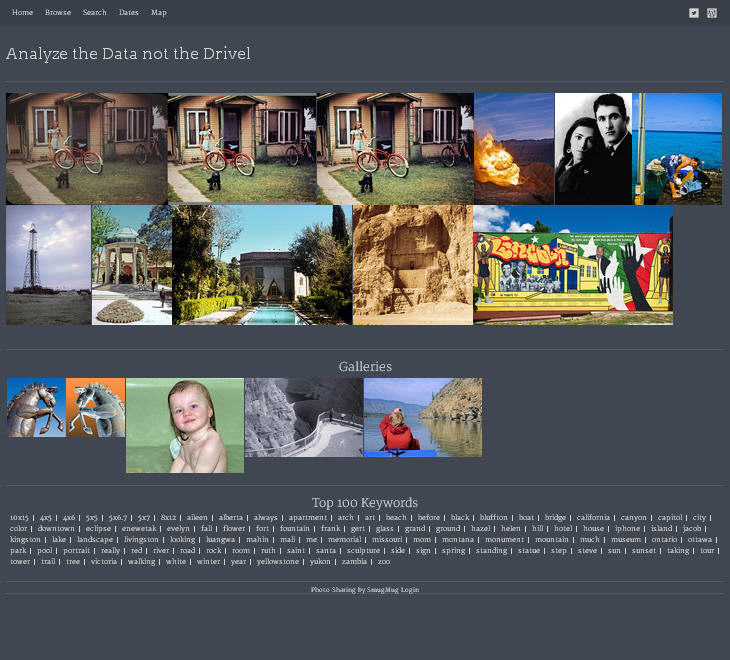
\includegraphics[width=0.23\textwidth]{newsmugss.jpg}
%\caption{~~~IMCAPTION~~~}
%\label{fig:4126X0}
%\end{floatingfigure}
%\end{figure}

%\captionsetup[floatingfigure]{labelformat=empty}
%\begin{figure}[htbp]
%\begin{floatingfigure}[l]{0.25\textwidth}
%\centering
%
\includegraphics[width=0.23\textwidth]{dilbert-attaboy.png}
%\caption{~~~IMCAPTION~~~}
%\label{fig:4126X1}
%\end{floatingfigure}
%\end{figure}



%\end{document}